\documentclass[9pt,usenames,dvipsnames]{beamer}

\usetheme[progressbar=frametitle,numbering=fraction]{metropolis}
\usepackage{appendixnumberbeamer}
\usepackage{booktabs}
\usepackage[scale=2]{ccicons}
\usepackage{pgfplots}
\usepgfplotslibrary{dateplot}
\usepackage{xspace}
\usepackage{algorithm2e}

%\usepackage[utf8]{inputenc}
%\usepackage{amsfonts} % For AMS Beautification
%\usepackage{fullpage} % For More Realistic Page Usage
%\usepackage{algpseudocode} % For algorithm layout
%\usepackage[boxed,ruled,vlined]{algorithm2e}
%\usepackage{bm}
%\usepackage{color}
%\usepackage{commath}
\usepackage{amssymb, amsmath, amsfonts,mathrsfs,amsthm}
\usepackage{mathabx} % \widecheck - inverse Fourier transform
\usepackage{mathtools}
\usepackage{graphicx} %includegraphics[scale=#]{filename}
\usepackage{float}
 \usepackage{relsize}
%\usepackage{pdfsync}
%\usepackage{hyperref}  
%\usepackage{upgreek}
%\usepackage[round]{natbib}
% \usepackage[backend=biber,style=numeric, citestyle=ieee]{biblatex}
\usepackage[style=apa]{biblatex}
\addbibresource{reference.bib} %Imports bibliography file

\usepackage[most]{tcolorbox}
\newtcolorbox{titlelessblock}{
  enhanced,
  boxsep=0.25ex,
  arc=1.25ex,
  opacityframe=.6,
  opacityback=.6,
  colback=white,
  %colframe=black!25!white,
  colframe =black!40!white,
  boxrule=0pt
}

\newcommand{\sdag}[1]{{#1}^{\dag}}
\newcommand{\Zee}{\mathbb{Z}}
\newcommand{\zee}{\mathfrak{z}}

\let\oldcite=\cite
\renewcommand\cite[1]{\hyperlink{#1}{\textcolor{blue}{\small{(\oldcite{#1})}}}}


\renewcommand{\footnotesize}{\scriptsize}

\newcommand{\themename}{\textbf{\textsc{metropolis}}\xspace}

\title{Waht's new in MPI-SPPY}
% \subtitle{A Bootstrap Approach}
\date{}
\author{David L Woodruff \inst{1}\\
  Jean-Paul Watson \inst{2}\\
  Ben Knueven \inst{3}}


\institute{\inst{1} Graduate School of Management, \\ University of California, Davis\\
  \inst{2} Lawrence Livermore National Laboratory\\
  \inst{3} National Renewable Energy Laboratory
}
% \titlegraphic{\hfill\includegraphics[height=1.5cm]{logo.pdf}}
\date{ICSP 2025}

\begin{document}

\maketitle


\metroset{sectionpage=none}

\begin{frame}{Optimization Under Uncertainty}

Today we will work with abstract problems such as:
\alert{
\Large
$$
\min_x h(x,\boldmath\Xi)
$$}
\begin{itemize}
\item $\boldmath\Xi$ is a random variable
\item The function $h$ captures constraints as well as any data modeled as known with certainty.
\end{itemize}
But the random variable necessitates some additional specification such as
requiring a form of robustness or perhaps...
\pause
\alert{
\Large
\begin{equation}
        \min_x E_{\xi\sim F}h(x,\xi)  \label{eq:TheProblem}
\end{equation}
}
Where the distribution $F$ is unknown and, of course, almost always unknowable. 
\end{frame}

\begin{frame}{Outline}
  \begin{itemize}
\item What is MPI-SPPY?
\item New communication paradigm
  \item New user interface.
\item New ways to interface with AMLs
\item If time...
  \end{itemize}
\end{frame}


\section{MPI-sppy}
\begin{frame}{MPI-sppy: The paper and the software}
\begin{itemize}
\item B. Knueven, D Mildebrath, C. Muir, JD Siirola, J-P Watson, DL Woodruff, ``A parallel hub-and-spoke system for large-scale scenario-based optimization under uncertainty,'' {\em MPC}
\item Find $\hat{x}$ with bounds and/or confidence intervals on the objective function for a scenario-based $T$-stage expected value problem with scenario set $\Xi$.
\end{itemize}
  
\end{frame}

\begin{frame}{MPI-sppy: The paper and the software}
\begin{itemize}
\item Find $\hat{x}$ with bounds on the objective function (and confidence intervals) for the problem solved to do that; generally scenario-based, e.g.:
  $$
   \min_x \frac{1}{N} \sum_{i=1}^N h(x, D_i).
   $$
   for some sample $D$ of size $N$.
  \begin{itemize}
  \item Software is available at \url{https://github.com/Pyomo/mpi-sppy}
  \item It is a library, but we also have a generic program (coming back toward PySP)
    \item It is designed for HPC, but does run on a laptop.
    \end{itemize}
\end{itemize}
\end{frame}

\begin{frame}{The Original Architecture}
  \subtitle{MPI: Message Passing Interface}

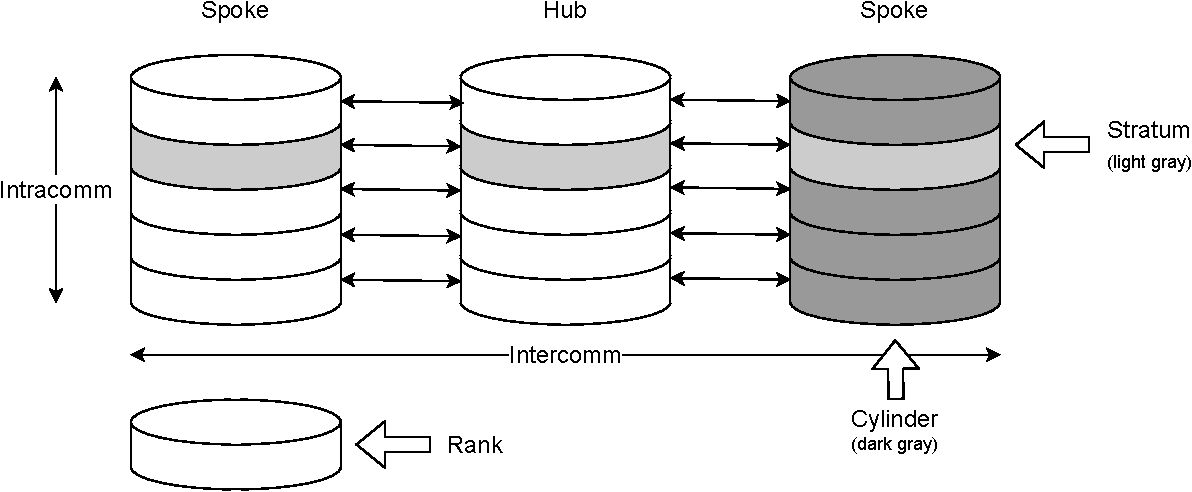
\includegraphics[width=1.0\linewidth]{hubspoke.pdf}
But the connections have changed
\end{frame}


\begin{frame}{Top View of Newer Version}

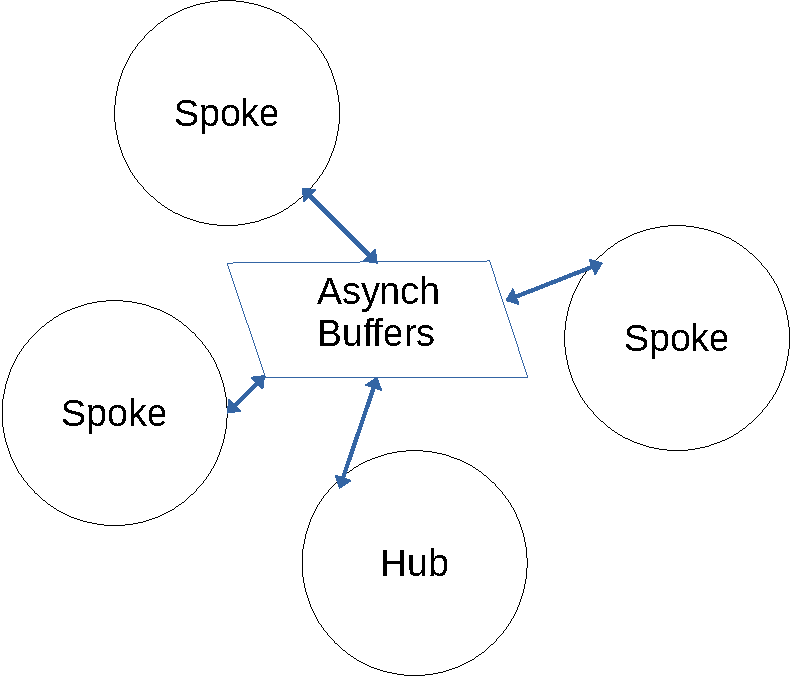
\includegraphics[width=1.0\linewidth]{topview.pdf}

\end{frame}

\begin{frame}{Changes}
xxxx the hub now just does some output and decides to shut down
\end{frame}



\begin{frame}{Agnostic to the AML}
  For scenario based decomposition...
  \begin{itemize}
  \item Loose:
    \begin{itemize}
    \item You code your AML to write an MPS (or maybe lp) file for each scenario along with a json file for each scenario that lists the nonanticipative variabes for each node in the scenario tree traversed by the scenario.
    \item You do this once and let mpi-sppy take over.
      \item No Python programming required (unless, of course, thats how interact with your AML)
      \end{itemize}
    \item[]
    \item Tight: If your ``AML'' is callable in the sense that an outside caller
      can modify the objective, then
      \begin{itemize}
      \item You hope we already have added support for your ``AML'' (we now have support for AMPL, GAMS, and GurobiPy)
        \item You need to write a thin wrapper in Python for your model
        \end{itemize}
  \end{itemize}
\end{frame}

\begin{frame}{More about loose coupling}
xxx
\end{frame}

\section{If time... Consensus ADMM Under Uncertainty}

\begin{frame}{Consensus ADMM Under Uncertainty}
  \begin{itemize}
  \item There is a paper with Aymeric Legros on OOL, but write to me for a somewhat better version.
  \item Today, I will give a brief overview, with almost no notation.
    \begin{itemize}
    \item You might want to do scenario decomposition for stochastics and you might want to do consensus ADMM decomposition because you have a huge problem (or you might be decomposing just to get parallel speed-up or for security reasons).
    \item We combine the two. Under the hood, the trick is the tree.
      \item But the interface is that you tell the software about your scenario tree for stochastics and about your consensus variables and subproblems for ADMM using wrappers for your model.
      \end{itemize}
    \item The software is available on github as part of MPI-SPPY.
  \end{itemize}
\end{frame}

\begin{frame}{A Simple Example}
  \begin{itemize}
  \item Consider a batch production/distribution problem with uncertain production yields
  \item Batch sizes must be non-anticipative, while shipping quantities, inventory etc. can depend on realized yields.
  \item Suppose the ADMM subproblems are regions with a few arcs between them.
    \item So there must be a consensus for flow on the arcs between two regions.
  \end{itemize}


\end{frame}

\begin{frame}{Progressive Hedging and the like}
\centering
 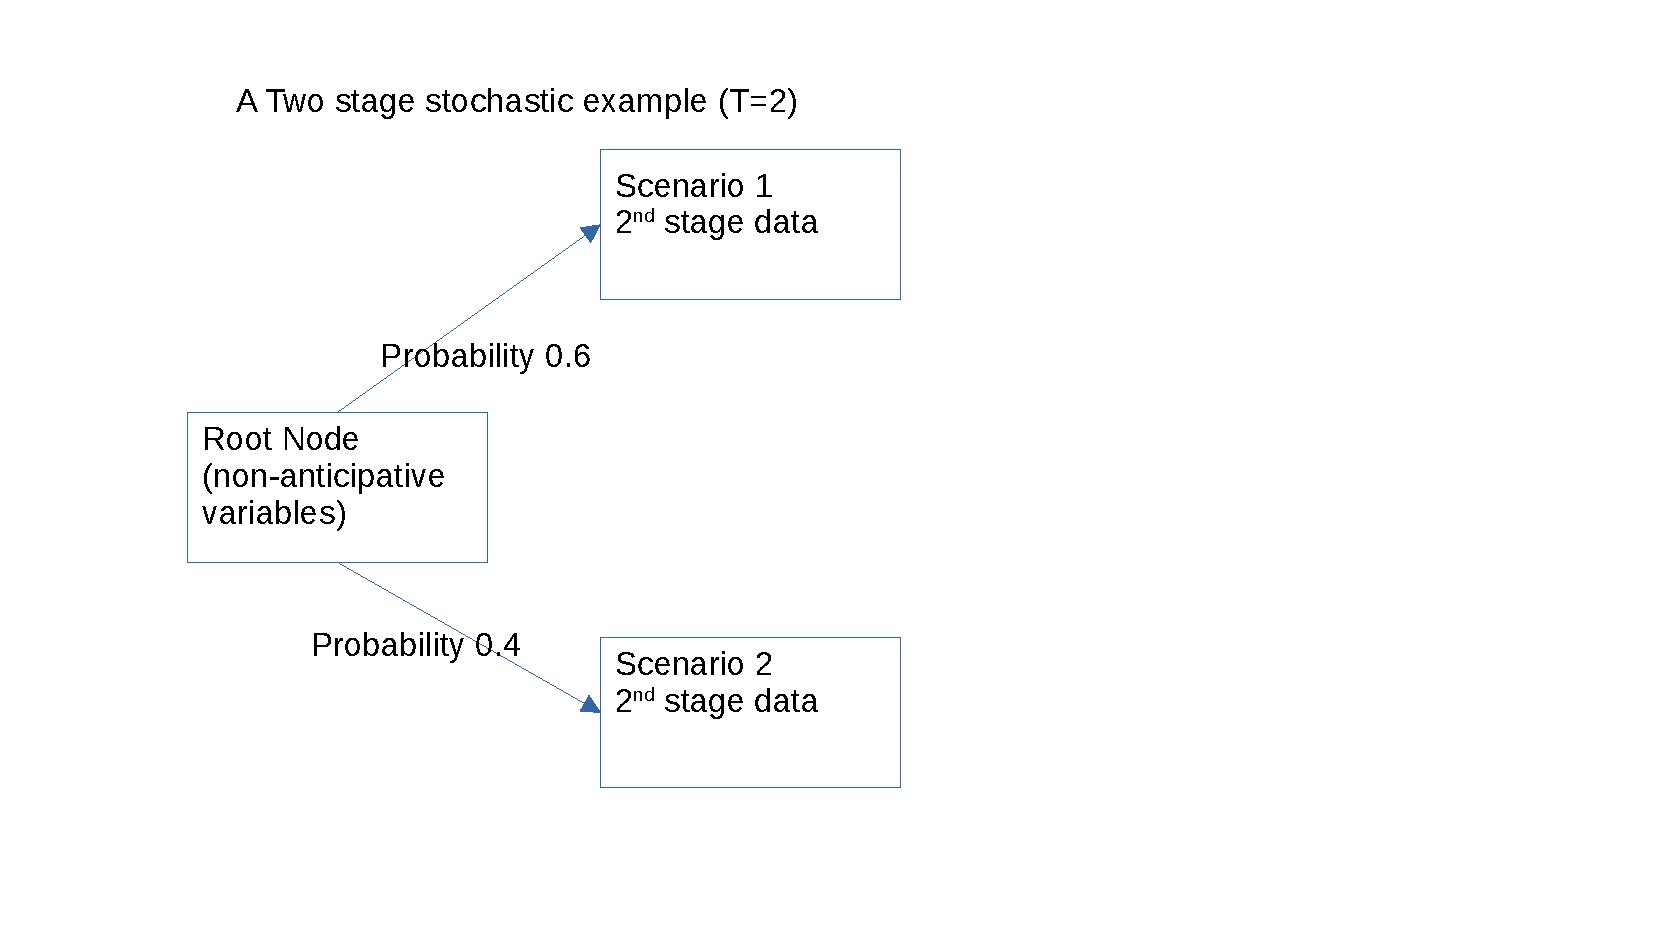
\includegraphics[width=1.1\linewidth]{tree1.pdf}
\end{frame}

\section{Extended Scenarios and Tree}
\begin{frame}{Under the hood: Extended Scenarios and Tree}
  \begin{itemize}
\item The collection of ADMM subproblems, $A$, are considered to emanate from a scenario tree node that is replicated for addition
  to the original scenario tree at every original leaf node.
\item So now we have a tree with $T+1$ stages and $|\Xi| |A|$ {\em extended scenarios}.
\item There's going to need to be some funny business with non-anticipative variables and with probabilities if we are going to use standard stochastic scenario
  decomposition algorithms.
\end{itemize}
\end{frame}

\begin{frame}{Combined ``Scenario'' Tree}
\centering
 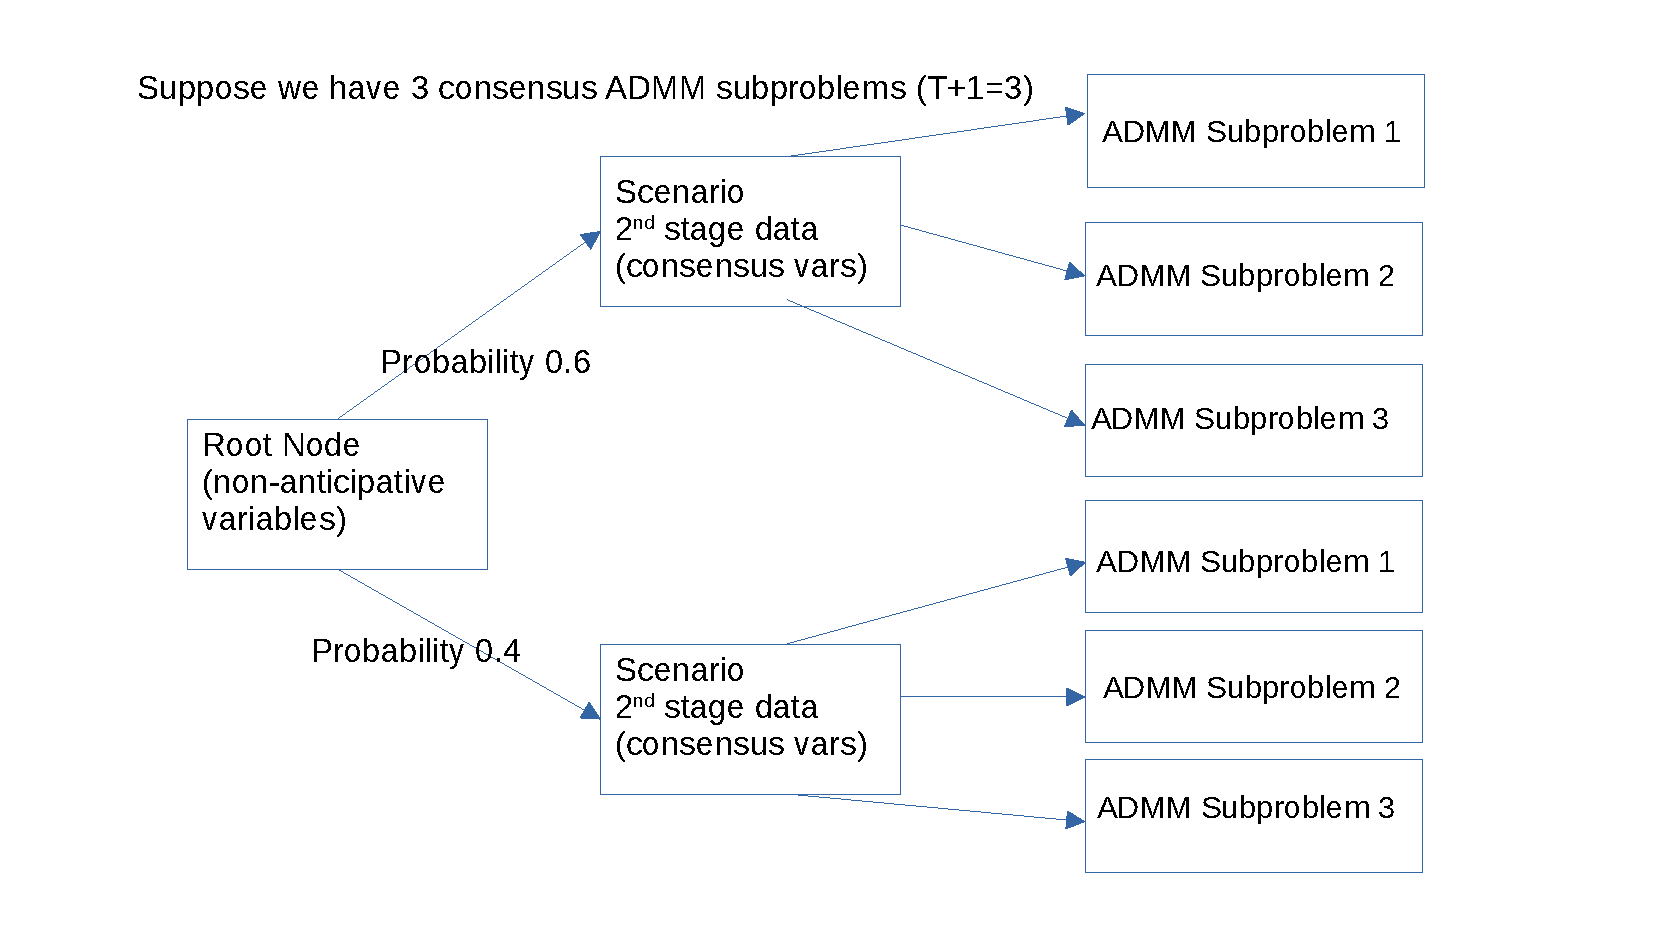
\includegraphics[width=1.1\linewidth]{tree2.pdf}
\end{frame}

\begin{frame}{Conclusions about Stochastic consensus ADMM}
\begin{itemize}
\item Our paper describes methods and software for using a stochastic programming decomposition algorithm for stochastic consensus ADMM.
\item You could use similar thinking to adapt an ADMM algorithm for stochastic ADMM.
\item Aside: decomposition seems to be needed for only a fraction of ``pure'' stochastic problems, so ADMM problems seem like a good place to hawk our wares.
\end{itemize}
\end{frame}

\end{document}

%%%%%%%%%%%%%%%%%%%%%%%%%%%%%%%%%%%%%%%%%



